\documentclass[a4paper]{article}

%% Language and font encodings
\usepackage[english]{babel}
\usepackage[T1]{fontenc}

%% Sets page size and margins
\usepackage[a4paper,top=3cm,bottom=2cm,left=2cm,right=2cm,marginparwidth=1.75cm]{geometry}

%% Useful packagess
\usepackage{amsmath}
\usepackage{graphicx}
\usepackage[colorinlistoftodos]{todonotes}
\usepackage[colorlinks=true, allcolors=blue]{hyperref}
\usepackage{hyperref}
\usepackage{float}

\title{Coding Standards}
\author{Triple Parity}
\date{}
\begin{document}
\maketitle

\graphicspath{{images/coding-standards/}}
% 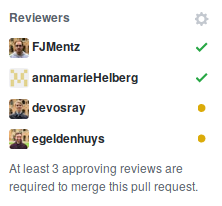
\includegraphics[scale=0.5]{github_3_reviews_required.png}

\section{Introduction}

This document gives a brief overview of the coding standards we plan on using in our project. 
To ensure consistency throughout our project we will cover how we will be designing our coding 
documents written in Angular (front end), and JavaScript (back end). We will be using TypeScript 
in Angular and therefore will be keeping the same coding standards for both front and back end 
JavaScript.

\section{Required and optional items}
\subsection{Naming Conventions}
In Angular 5 we generate components inside the project. Each Component contains a single HTML, CSS, Spec and 
TypesScript file. To ensure consistency across all file names when creating a component Angular 
Components use only lower case letters and in any case where there are multiple words separate each 
with a "-" ie. "stack-view";\newline
In Angular 5 we also generate our own Modules which we can use to represent a JSON object of variables we can pass 
too and receive from the docker API. To keep consistency, Modules should be created in the same way as Components. ie. "stack" \newline
We also make use of Angular 5 Services which we use to help us make an asynchronous system. When creating a Service we should 
keep to the same naming conventions as Modules and Components. It is also required to append the word service ie. "stack-service" to a service. 
It is Import to Note that Angular generates Components, Modules, and Service objects with capital letters and camel 
casing but we would prefer file names to remain lower case and the actual Component being passed around by Angular to 
remain Capitalized with camel casing.
\newline\newline
Function names inside TypeScript files will always start with a lower case letter, if the function requires more 
than one word it will make use of camel casing ie. "getStack()". 
Attributes and local variables will follow the same naming conventions as functions. 
\newline 
Objects inside each module must always start with a capital letter. 
\newline\newline
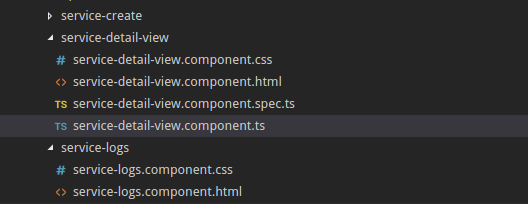
\includegraphics[scale=0.5]{file_name.png} \newline\\
Above is a view of the file names of the service-detail-view component. 



\subsection{Layout rules}
Our group members make use of the Visual Studio Code IDE. 
Every TypesScript file is put through a series of tests, one of which is a lint test. This is a test to see if the 
file's contents are maintained by coding standards set up by the lint document. By making use of 
the TSLint tool \href{https://palantir.github.io/tslint/}{TSLint Website} we can set up VScode to display linting 
errors as errors a compiler would normally show, thus we are able to test and ensure coding standards across
our system.\\\\
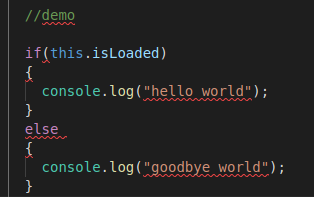
\includegraphics[scale=0.5]{TSLint_error.png} 
\qquad\qquad\qquad
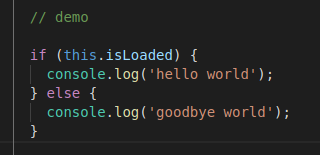
\includegraphics[scale=0.5]{TSLint_clean.png} \\
Above left is an example of what a developer will see if they develop using the wrong coding standards. 
Above right is an example of what the developer will see if they use the correct coding standards using VScode as the IDE.
\newline\\ 
\underline{A partial List of our coding standards:} 
\begin{itemize}
	\item Enforce return statements in getters
    \item Disallow assignment operators in conditional expressions
    \item Disallow constant expressions in conditions
    \item Disallow duplicate arguments in function definitions
    \item Disallow empty block statements
    \item Disallow irregular whitespace outside of strings and comments
    \item Disallow unreachable code after return, throw, continue, and break statements
    \item Enforce the use of variables within the scope they are defined
    \item Enforce that class methods utilize this
    \item Require default cases in switch statements
    \item Require the use of === and !==
    \item Disallow the use of eval()
    \item Disallow fallthrough of case statements
    \item Disallow new operators with the Function object
    \item Disallow new operators with the String, Number, and Boolean objects
    \item Disallow variable redeclaration
    \item Disallow javascript: urls
    \item Disallow assignments where both sides are exactly the same
    \item Disallow comparisons where both sides are exactly the same
    \item Enforce consistent brace style for blocks
    \item Require newline at the end of files
    \item Require newline at the end of files
    \item Enforce the consistent use of either function declarations or expressions
    \item Disallow trailing whitespace at the end of lines
    \item Enforce consistent line breaks inside braces
    \item Require semicolons instead of ASI
    \item Require let or const instead of var
    \item Enforce max characters per line
    \item Enforce the consistent use of single quotes in JSX attributes
\end{itemize}
These are the coding standards for all the Typescript files in the front end and are enforced by lint 
testing. Any git commit is first run through a lint test to ensure that the code is written according to 
these standards layed out. There are more see  \href{https://eslint.org/docs/rules/ }{ESlint rules}.
\\
For formatting we make use of the Prettier tool \href{https://prettier.io/}{(view site)} which helps remove blank wasted spaces and enforces a 
consistent level of indentation across all HTML, Typescript, and CSS pages.
\\\\

\subsection{Commenting practices}
Comments will be placed above complex functions or above service return function's. Any function that returns 
data should have a comment describing what the data type is of the data returned, unless it is a simple get
function. TODO:'s + ( + developers name + ) must be placed by a developer who has knowledge in a specific area of
code. This is not a promise that the developer know's everything but rather used as a temporary marker left by a developer 
to say that they will get back to or that they are stuck and require some help or possibly even to pass on the task to 
someone else. The developer should be able to provide other members with input about that piece of code at a later 
stage. \\
Enforce a space between comment expression and comment   



\section{FIle Structure}
As mentioned at an earlier stage in this document our project makes use of Angular and Components. 
A single Component is made up of 4 files\\ 

\includegraphics[scale=0.5]{component.png}\\
\begin{itemize}
	\item A CSS file
    \item A HTML file
    \item A Spec file
    \item A Typescript file
\end{itemize}
\pagebreak
We group all Components that share a type ie. Services together with one another in a directory of that type ie. Services\\
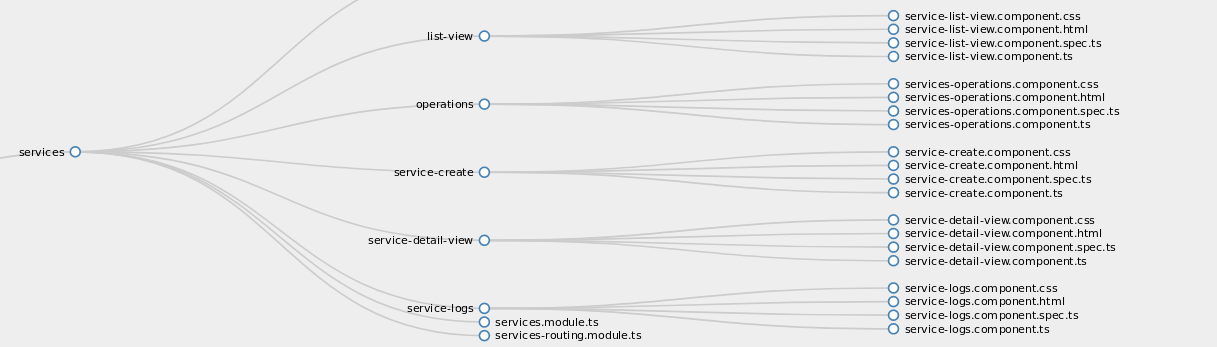
\includegraphics[scale=0.4]{service_directory.png}\\
In each of these directories are two very specific Modules. The first is a module used to import all the components 
that the all the other components of type "Service" --for example-- needs. This module has the same name 
as the directory. The second is a routing module, the module that sets up the links between the module and how 
to navigate the router to each component in that module.\\
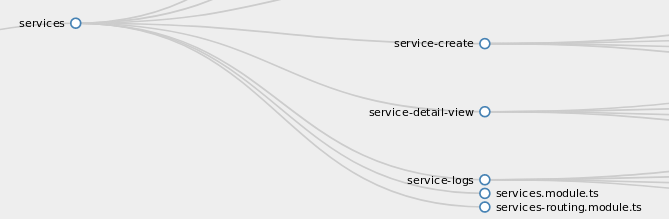
\includegraphics[scale=0.4]{routing_modules.png}\\
(this is a close up on the previous image)\\\\
There are 13 directories in the "pages" directory. The pages directory houses all the components that are 
displayed as a page in the interface. These include:
\begin{itemize} 
    \item home 
    \item login
    \item networks
    \item nodes
    \item page-not-found
    \item stacks
    \item services
    \item tasks
    \item volumes
    \item user-management
    \item webhooks
\end{itemize}
\pagebreak
A sibling to the pages directory is a the shared directory which contains components that are likely to be 
used across pages ie. the navbar\\
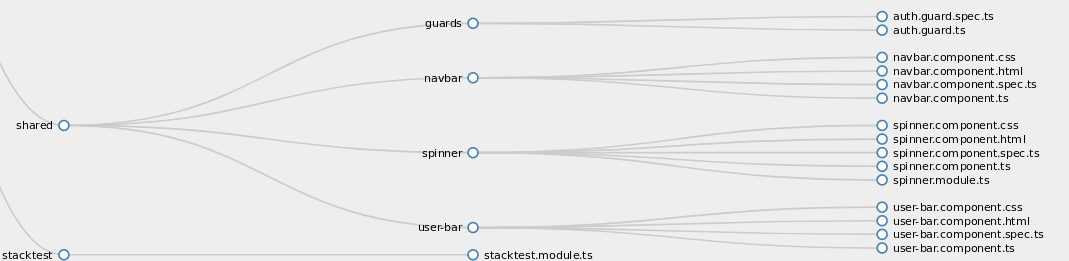
\includegraphics[scale=0.4]{shared.png}\\\\
Other siblings of the pages directory include the Module and Service (Not to get confused with the service component, 
services are used in Angular for requesting services) 
directories which contain all Modules and Services used by our system.\\
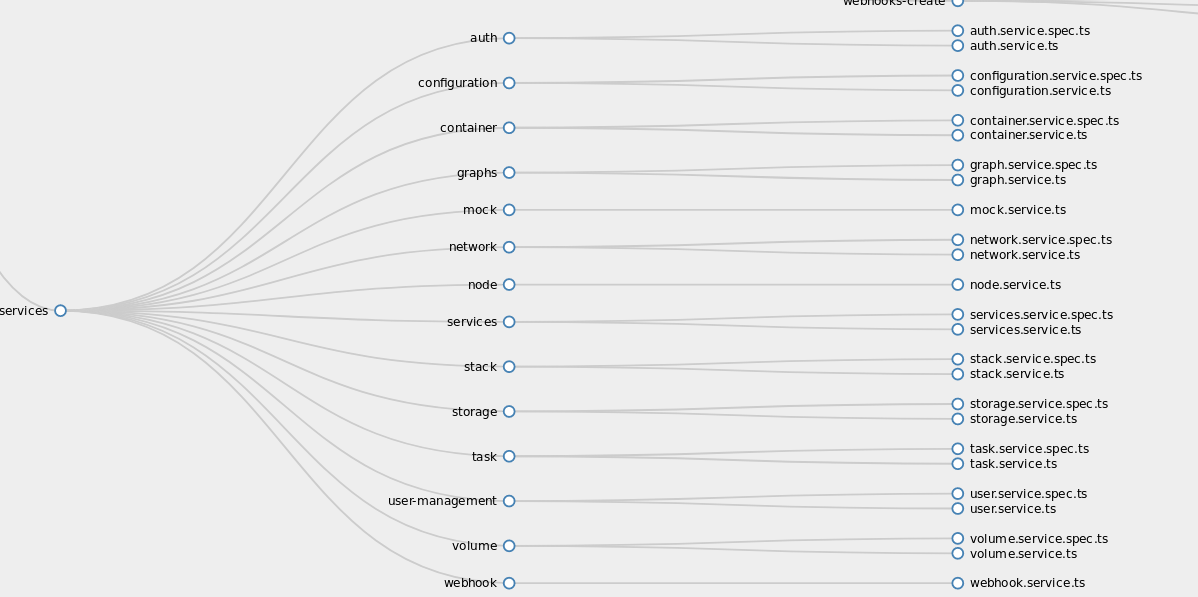
\includegraphics[scale=0.4]{service.png}\\\\\\\\
A complete view of our system can be seen on the next page\\ 

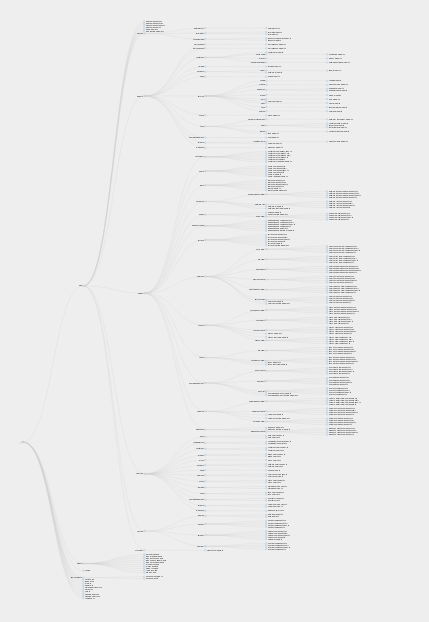
\includegraphics[scale=1]{system.png}\\

\section { Code reviews }
\subsection { Peer Reviews }
We make use of multiple peer reviews before merging any new code into git. A minimum of two group members 
must review code before it makes it's way into production. All new feature branches created by group members 
have to pass a series of travis build tests as well as linting tests mentioned earlier. After that they still 
have to be reviewed by peers before being merged into our develop branch. \\
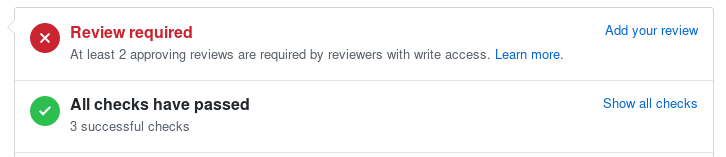
\includegraphics[scale=0.6]{reviews.png}\\
Besides peer reviews we also make use of lint testing as mentioned above which regularly monitors the coding 
standards of each commit. Commits that fail lint do not pass the tests and cannot be merged into develop.

\section{UML diagram}
\subsection { Docks UML }
With a system this large there are not many tools we can use to create an accurate uml diagram.
The following is the best we could find.\\

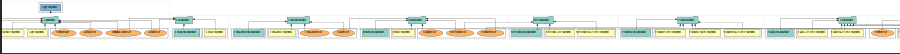
\includegraphics[scale=0.5]{uml.png}\\
\end{document}